\Section{Контекстные меню (Contextual menus)}

\Subsection{Контекстное меню}\\

    Контекстное меню создается при долгом нажатии на экран.

    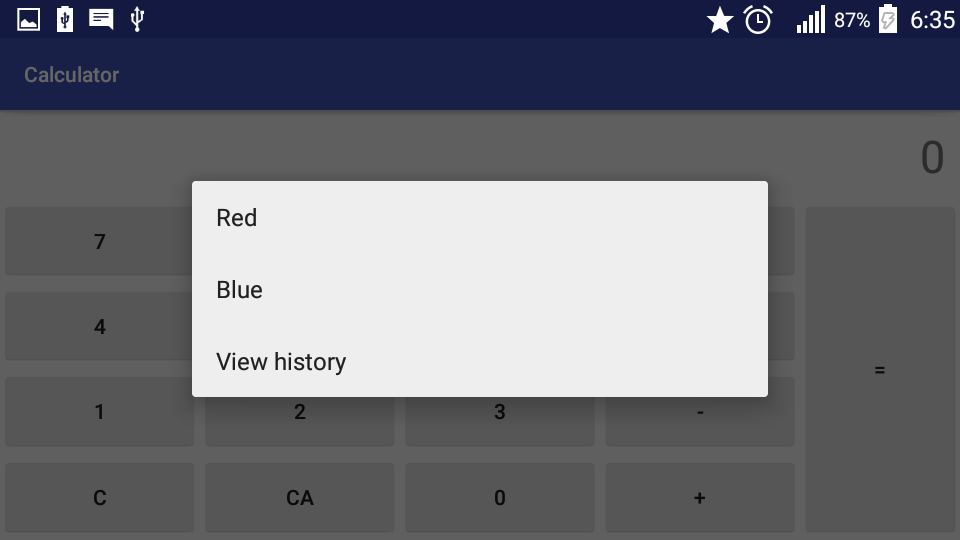
\includegraphics[scale=0.3]{06-context-menus/Screenshot.png}
    
\Subsection{Создание контекстного меню}\\

    Чтобы создать контестное меню, нужно в классе, соответвующем текущей Activity: 
    
    \begin{itemize}
        \item Вызвать метод registerForContextMenu(View view$\_$i);
    
        Хотим чтобы появлялось контекстное меню при долгом нажати на view$\_$i.
    
        \item Создать обработчик onCreateContextMenu, который будет вызываться каждый при открытии контекстного меню.
    
        void onCreateContextMenu(android.view.ContextMenu menu, view$\_$i, ContextMenuInfo menuInfo);
        
        где, 
        \begin{itemize}
            \item menu -- то, куда добавим пункты.
            
            оно при каждом вызове onCreateContextMenu новое. 
    
            \item view$\_$i -- элемент экрана, для которого вызвалось контекстное меню.
        \end{itemize}
    \end{itemize}

    \pagebreak
    \javacode{06-context-menus/onCreateContextMenu.java}

\Subsection{Обработка событий контекстного меню}\\

    Для обработки события выбора пункта меню добавим метод
    boolean onContextItemSelected(MenuItem item);
 
    \javacode{06-context-menus/onContextItemSelected.java}

\Subsection{Создание контекстного меню из макета (.xml)}

    Пусть xml файл лежит в app$/$res$/$menu$/$context$\_$menu.xml

    \pagebreak
    \xmlcode{06-context-menus/XmlMenu.xml}

    XML меню часто удобней: описыватся, как и большая чать UI в *.xml; меньше думаешь об ID.

    Создание menu из xml выглядит коротко:

    \javacode{06-context-menus/onCreateContextMenu2.java}

    Обработка выбора пункта аналогична:

    \javacode{06-context-menus/onContextItemSelected2.java}
